\chapter{Conclusion}

We now review the body of evidence from the previous Chapters to determine if they indeed shed light on 

One of the primary determinants of a merging system's fate is whether or not its remnant has a centrally peaked temperature.  While earlier simulations (\citeal{loreig09}) suggested a centrally peaked temperature, our own 

Mergers

- no longer get really hot in their centres.  The older simulations that vk10 based their ideas off of assumed approximate and irrotational mergers with large artificial viscosities.  Our SPH scheme gives similar (if somewhat cooler (Sec compare with Loreig) results), but other codes that are synchronized and use accurate initial conditions do not (check raskin+12 and dan+14 profiles?)  In particular, dan compares their simulations to ours, and find that their similar mass mergers mix less and (consequently) are hottest at their surfaces.

- while the arepo simulations are quite similar to the gasoline ones, this is the big difference between our two simulations: the 0.625-0.65 Msun merger in Gasoline is evenly heated, while the dense core is in Arepo is not, and remains much colder.  In the case of a purely hydrodynamic evolution even in Arepo there's no obvious way to heat the core other than adiabatic compression.  the core no longer mixes during this phase, so there's no way of bringing hot gas to the deep interior of the core.

-Diff between exact and approximate initial conditions is covered SEVERAL TIMES in our paper, as well as in Dan+14.  READ THESE FOR GOD'S SAKE!

- this leaves two problems:
	- is central ignition no longer possible?  perhaps not - synchronized mergers don't do it, and dan notes that his mergers are at least partly unsynchronized by the time they merge.
	- if not, how off center will any ignition occur?  This is difficult to say, and unfortunately depends both on the initial conditions of the WD 
	- thus, our mergers are likely 

-jI+13 non-local heating through magnetic reconnection?  compression looks mostly to be adiabatic, except near the very end (though they do see a trend of INCREASING temperature toward the center with resolution)

- We lastly stress the importance of observational work in this field: we've noted that sub-Mch merger remnants should become massive WDs, but the space density of these, and a comparison of these values to estimated merger rates from population counts and population synthesis, will give us a much better handle.  Their mass range will do so also, at least with providing a minimum cutoff for things that can explode (we note that there's poorly constrained wind mass loss)

\begin{figure}
\centering
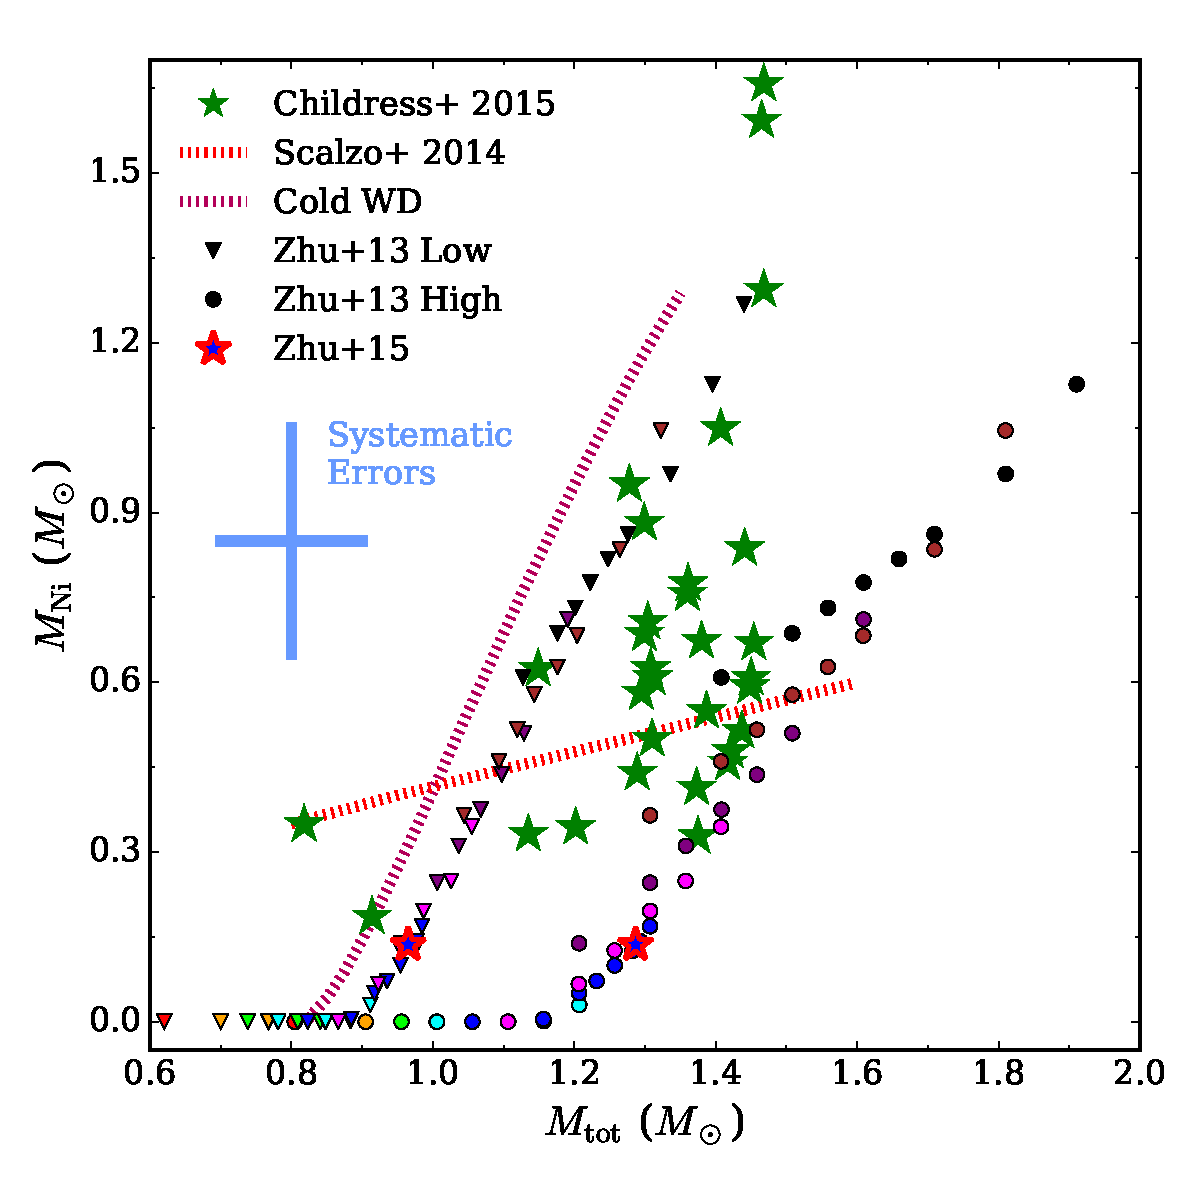
\includegraphics[angle=0,width=0.6\columnwidth]{conclusion/figures/c_MNi.pdf}
\caption{Relationships between total ejected mass \Mtot\ and synthesized \Ni\ mass \MNi\ for adiabatic and \dnabconv-inclusive WDs that experience a pure detonation immediately after the end of simmering, estimated using \cite{sim+10}.  Also plotted are the \Mtot\ and \MNi\ yields of $31$ observed SNe Ia from \cite{chil+15}, and the relationship derived by \cite{scalzrs14} from 337 observed SNe Ia.  \cite{chil+15}'s systematic error bars, indicating how much their values can be shifted in unison, are also included.  The dashed magenta line is the relationship for the pure detonation of cold (uniform $10^5$ K) WDs, with the simulation results of \cite{sim+10} overdrawn.}
\label{fig:c_mcmce_mni}
\end{figure}

%-resummarize all papers
%-don't say what we used to think

%-MRI growth rate in remnant?
%-simulation code does matter for post-merger evolution (hydrodynamic waves, magnetic fields)
%-

%\section{Does the \citeal{vkercj10} Channel Work?}

%Even if we assume runaways are vertical, the typical spun-down remnant still doesn't get to 1e7 gcc!

%%This result poses a problem for the \citeal{vkercj10} sub-\Mch\ merger channel.  \cite{shen+12} finds further compression could occur during the subsequent \textit{thermal} evolution of the remnant over $\gtrsim10^4\,\mrm{yr}$, which may allow more remnants to reach higher central density and enclose more mass within their cores.  Whether central burning could still begin is uncertain, however, since thermal diffusion and neutrino-driven cooling may favor off-center carbon ignition, or simply net cooling, even for those post-viscous remnants that are initially $\gtrsim5\times10^8\,\mrm{K}$ at their center.  Moreover, remnants, with radiation-dominated and highly magnetized carbon atmospheres, will likely drive strong outflows during their thermal evolution, further complicating predictions.  We note one advantage for delaying the explosion to during thermal evolution is the removal of the ``clutter'' of the $\gtrsim0.1\,\Msun$ hot envelope surrounding the core and extending out to $\gtrsim10^{11}\,\mrm{cm}$ \citep{shen+12}.  This imparts signatures onto the explosion not seen in ordinary SNe Ia, such as a double-peaked light curve from the shock cooling of the envelope, excess blue and UV emission prior to peak light, and a slow-decaying light curve near peak light \citep{frye+10,levasg15,pirom15}.  While \cite{shen+12}'s simulation suggests thermal evolution will do little to alter the overall structure of the envelope \citep{pirom15}, it does not account for mass loss due to winds.  These will significantly alter the size and structure of the envelope, perhaps mitigating its effects on any eventual explosion.  Meanwhile, material ejected from the remnant (both during its viscous and subsequent thermal phases) moving at the escape velocity will approach $\sim10^{17}\,\mrm{cm}$ after $\sim10^4\,\mrm{yr}$.  Interaction between this material and light from the supernova could explain \citep{shen+12, ji+13} observations of SN Ia-CSM interactions such as time-variable NaID lines (eg. \citealt{pata+07, simo+09}).

%% Magnetic coupling between the outflow and the remnant will aid in its spindown and possibly generate non-local heating through magnetic resistivity.

%Is the classic Mch DD channel even possible?

%-
%-





%\section{Observable Counterparts to Mergers}

%\section{The Evolution and Appearance of Quiescent Merger Remnants}

%\cite{schw+16} also consider in depth the observable properties of their $\1.5\,\Msun$ merger remnant (undergoing carbon and neon burning) in \mesa.  They note that the luminosity of the nuclear burning zone is almost entirely carried away by neutrino losses (as the burning zone sits at the $\taucc = \taunu$ line), and so the remnant's source of luminosity is the heat from the merger and viscous evolution.  Since sub-\Mch\ remnants have the same order of magnitude total energy as \Mch\ ones, their observed properties will likely be similar.  The find that, with an envelope and a radiation-dominated hot atmosphere of $10^{12}-10^{13}\,\mrm{cm}$, the remnant initially radiates of order the Eddington luminosity for a $1.5\,\Msun$ star ($\sim10^5\,\Lsun$) and has a photospheric temperature ranging from $4000 - 10^5\,\mrm{K}$.  These are very similar to the values \cite{shen+12} find in their thermal evolution simulation.

%The above values, however, do not account for winds.  Early-on during the thermal evolution, the low temperature of the outermost remnant layers coupled with a CO-composition will lead to dust generation, which will subsequently be launched as a wind.  \cite{ji+13} also find that much of the remnant envelope volume (though not mass) becomes marginally magnetic pressure-dominated ($B^2/8\pi P_\mrm{gas} \sim 1$), and that the remnant magnetically drives bipolar outflows, adding to the outflux of material.  \cite{schw+16} estimates this may drive the photosphere out to $\sim10^{15}\,\mrm{cm}$, with corresponding photospheric temperatures of $\sim500\,\mrm{K}$, and lead to RCrB-like variablility in the remnant's luminosity.  As noted previously, given the similarity of this system to the cores of post-AGB stars, these winds may also lead to the loss of a substantial fraction of the remnant's mass, which significantly complicates the thermal evolution process (see \cite{schw+16} Sec. 4).

%% Shen+12 gives the escape velocity at 10^13 cm as 60 km/s.  Given 10^4 years of evolution, this wind could transport material to 10^18 cm, possibly explaining the variable sodium emission.

%\section{The Influence of Merger Remnants Properties on Potential Explosions}

%If sub-\Mch\ CO WD merger remnants indeed trigger thermonuclear detonations following post-merger viscous evolution, will these explosions resemble SNe Ia?  As noted in the introduction, SNe Ia observations and radiative transfer models for explosions are now sophisticated enough to distinguish fine details between different progenitors.  This question has been taken up by a number of theorists \citep{frye+10, shen+12}  Shen+12 conclusions!

%\cite{frye+10} and \cite{rask+14} do simulations

%\begin{itemize}
%	\item What are the mass loss rates of non-explosive mergers due to carbon dust superwind?  can we estimate?  could it possibly lead to Kepler's 0.6Msun oxygen WD? Shen+12 (Just under Eqn. 7) note that mass loss in radiation-dominated H/He-deficient envelopes is poor. %http://adsabs.harvard.edu/abs/2016Sci...352...67K
%	\item Near-eddington carbon burning star?  See Sec. 4 paragraph 1 of Shen+12.
%	\item Discussion with Marten: while we can't rule out further compression leading to nuclear burning during the thermal evolution phase, a combination of magnetically and Eddington-launched outflows will make the surroundings very messy - write more about this in SN Ia appearance stuff.
%	\item Importance of Ia-CSM stuff?  Shen+12 and Ji+13 (Sec. 2.2.3) have extensive sections on it.
%	\item Ji+13 has a mean magnetic field of 2e8 G; what does our simulation have?  They also (bottom of pg 7) give a quick estimate for magnetic lifetime.
%	\item What's the difference between a ring of material at $10^{13}$ cm and a continuous envelope that ends at the same radius?  Does one resemble Ia-CSM interaction, but the other lead to Fryer+10 or Piro+15 early time brightening?
%	\item Even super chandra DD systems will be much less dense than their WD binary progenitors - consequences for explosions?
%\end{itemize}



%\section{Avenues for Future Exploration}


%\subsection{Future Simulations of Mergers and Post-Merger Evolution}

%Do we need to simulate more merging WDs, especially using novel magnetohydrodynamic schemes?  Ch. STUFF suggests that the hydrodynamics up to coalescence and overall remnant properties do not substantively change when transitioning from simulating with a traditional variant of SPH to doing so with a modern moving mesh code, and getting the initial conditions (eg. synchronization, accurate tidal bulges for the onset of mass transfer) right is likely to be more important.  We await results from the the Eulerian grid WD merger simulations of \citep{katz+16} for further confirmation.

%What does require further work is the magnetic evolution during the merger, as well as the early phase of post-merger evolution and further magnetic field growth following coalescence.  The former has been insufficiently investigated with the latest generation of MHD codes, which may end up predicting very different field configurations (and possibly energies) than our exploration of the problem with \arepo.  The latter, however, is not only also poorly explored (only one group has conducted a full MHD simulation!) but essential to better understanding post-merger evolution.  This regime is particularly challenging for codes, since it requires the code minimize numerical hydrodynamic and magnetic viscosity (traditionally problematic for SPH codes) while maintaining conservative quantities -- particularly angular momentum -- over hundreds of dynamical times (traditionally difficult for grid codes).  Moreover, the problem is stiff, since evolution occurs both on a dynamical (with spiral waves) and viscous timescale, and thus quite computationally intensive.  We note the recent introduction of two codes: duffel's and hopkins', that could potentially bridge the gap.

%Arepo MHD doesn't do a good job of conserving angular momentum - balance plot shows it spurious gains it.  May be due to divergence cleaning (hopkins 16)


%Simulations of detonations within violent mergers (eg. \ref{pakm+10, bull+16, krom+16}) or mergers shortly after coalescence \citep{rask+14,vros+15}, do not reproduce the light curves and spectra of SNe Ia.  

%OUR REMNANTS AREN'T RADIATION DOMINATED.  Prad/Pion \propto T^3/\rho \propto \rho in adiabatic envelopes; we're in general much colder for any given density than Shen+12, so in fact we don't have radiation dominated envelopes, but we still have extended ones!

%Shen+16 is important, since nuclear burning energy doesn't get to exterior before 1e4 years are up, so non-burning remnants will look similar!


%krom+16 http://adsabs.harvard.edu/doi/10.1093/mnras/stw962
%bull+16 http://adsabs.harvard.edu/abs/2016MNRAS.455.1060B
%vros+15 http://adsabs.harvard.edu/abs/2015arXiv151004286V

%papi+15 http://adsabs.harvard.edu/abs/2015MNRAS.449..942P

%NEW CODES:
%http://adsabs.harvard.edu/abs/2016arXiv160503577D
%http://adsabs.harvard.edu/abs/2016MNRAS.455...51H

%http://adsabs.harvard.edu/abs/2016ApJ...816L...9O

%http://adsabs.harvard.edu/abs/2015arXiv151203442P
%http://adsabs.harvard.edu/abs/2016MNRAS.tmp..977F
%http://adsabs.harvard.edu/abs/2016ApJ...818...26D

%http://adsabs.harvard.edu/abs/2016arXiv160401021F
%http://adsabs.harvard.edu/abs/2016ApJ...818L..19M

